\section{Analyse de l'existant}
\subsection{Erco.xyz \cite{Erco}}

Erco est un outil initialement développé à l'Université de Lorraine facilitant la configuration  des routes réseau avec Exabgp en réécrivant une partie du fichier de configuration d'Exabgp. Erco fournit une API RESTful et une interface web utilisateur. L'interface web permet de facilement : annoncer un nouveau réseau ou IP, modifier ou supprimer une route, envoyer des commandes à Exabgp( reload, show routes show neighbors et version).\\
L'esthéthique et les fonctionnalités de cette interfaces web sont utile pour notre projet. En effet, les bouttons "Relancer Exabgp" et "Exabgp fonctionne" sont exactement se que l'on a besoin. De plus notre section "lancer commande" ressemblera à celui de Erco mais avec plus de commande exécutable et un retour de message de Exabgp plus précis pour chaque commande. Nous prendrons aussi exemple sur Erco pour executer les commandes avec arguments sous forme de formulaire, et afficher les routes sous forme de tableaux, de liste. 
\\
\\
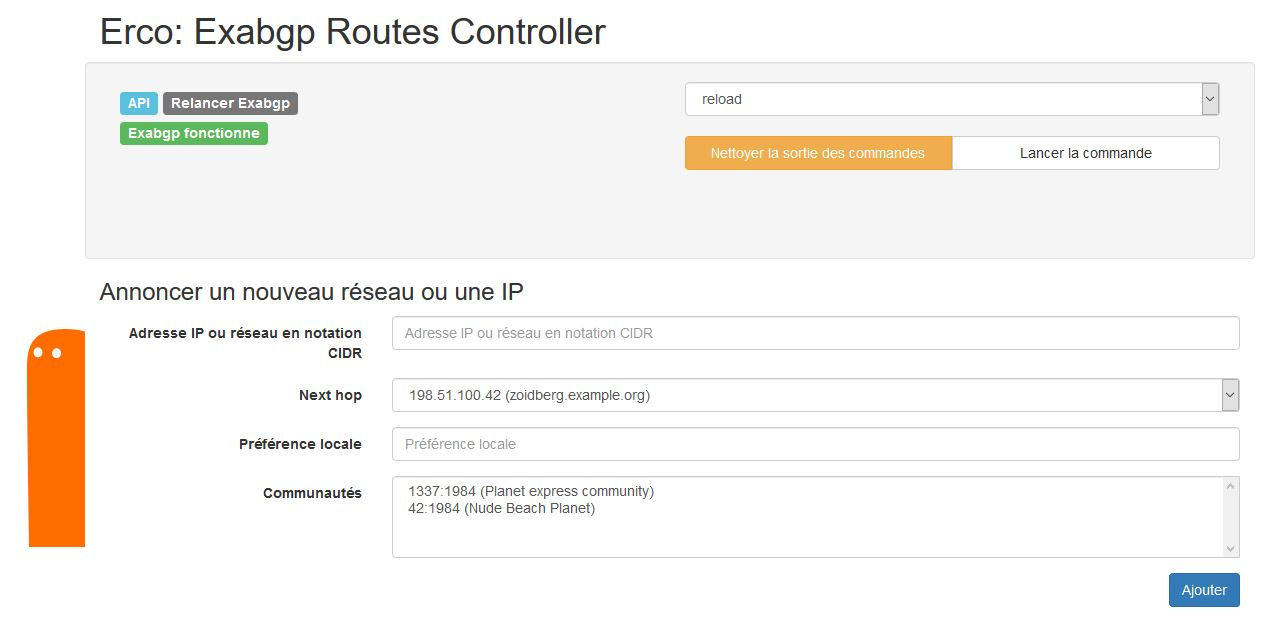
\includegraphics[scale = 0.5]{img/erco1.JPG}
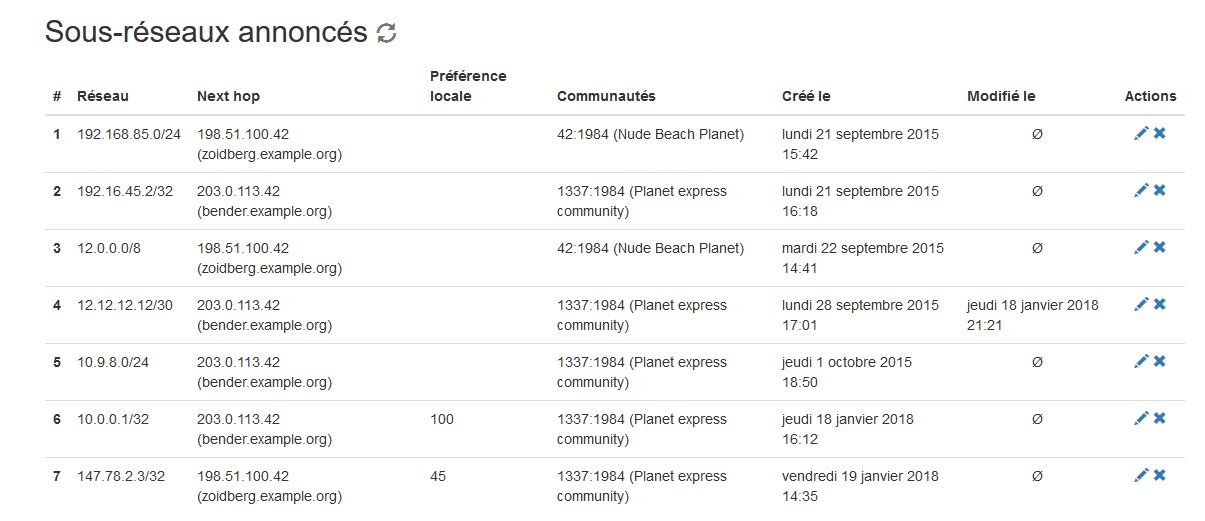
\includegraphics[scale = 0.5]{img/erco2.JPG}

\subsection{ExaBGPmon}
ExaBGPmon est une interface web sur le même principe que Erco.xyz, mais nous n'allons rien retenir de se site car il est moins intuitif et ergonomique que Erco et propose les mêmes fonctionnalités.
\\
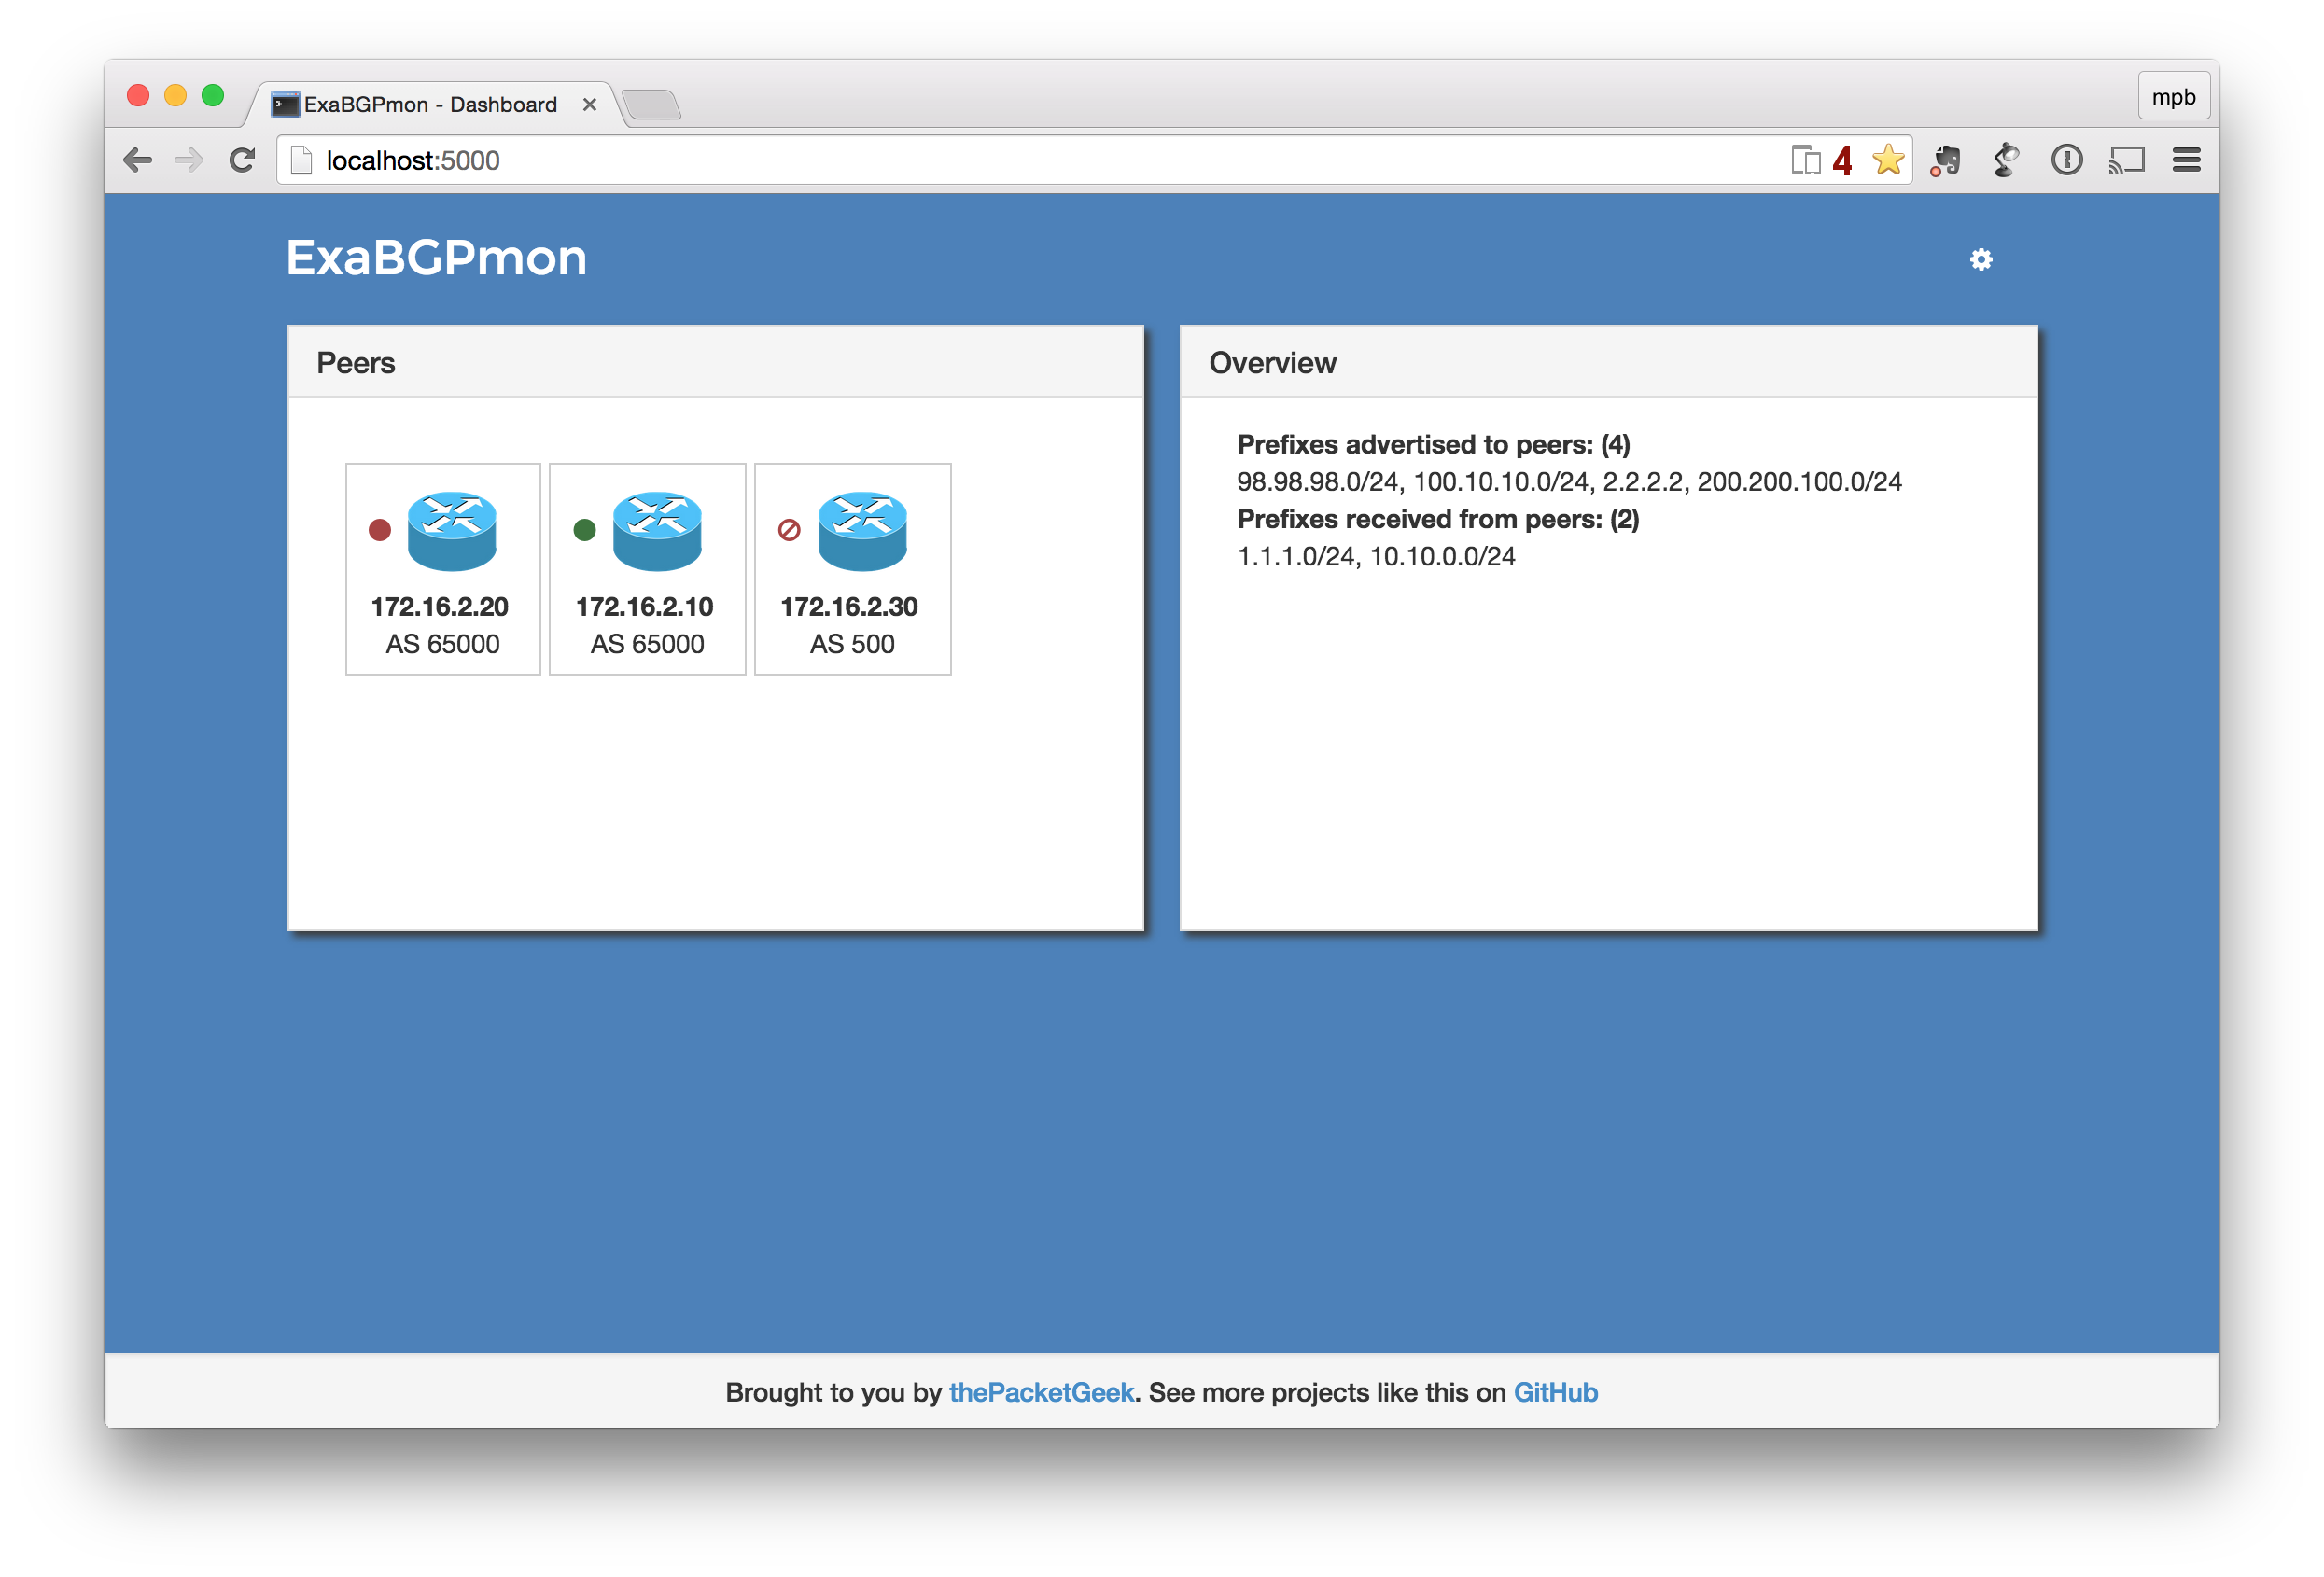
\includegraphics[scale = 0.40]{img/exabgpmon.png}


\subsection{ExaBGP}
ExaBGP est un outil open source écrit en Python qui permet d'interagir avec les réseaux BGP. Le logiciel peut injecter des routes annoncés dans les réseaux. 
ExaBGP offre un API contenant plusieurs commandes afin de manipuler les routeurs BGP. On peut aller voir la liste des commandes dans l'API d'ExaBGP : 
\\
\\
\url{https://github.com/Exa-Networks/exabgp/wiki/Controlling-ExaBGP-:-interacting-from-the-API}
\\
\\
Et apprendre à l'utiliser avec les tutos suivants:
\\
\\
\url{https://thepacketgeek.com/series/influence-routing-decisions-with-python-and-exabgp/}

\subsection{Meteor.JS \cite{Meteor.JS}}
\begin{center}

\includegraphics[height=1cm]{img/Meteor-logo.png}
\end{center}

Meteor.JS est un framework open-source javascript, Node.JS qui permet l'élaboration d'une application web de type RESTful. Elle permet de développer le client et le serveur de l'application web avec le même langage.\\
Notre client voulait une interface web développé en JavaScript de type Restful. Pour un déploiement et implémentation plus rapide de cette interface nous avons décidé d'utiliser le framework open-source Meteor.js qui réponds à ses besoins. De plus avec la possibilité d'utiliser des packages (extensions) de meteor.js nous pouvons implémenter certaines choses plus rapidement.\\
\\
Les packages utilisés sont:
\begin{itemize}
\item twbs:bootstrap
\item ian:accounts-ui-boostrap-3
\item iron:router
\end{itemize}

%client javascript RESTfull, nous plus facile package, serveur cache client.
\vspace{0.5cm}
Voici quelques liens pour pouvoir s'informer plus sur Meteor.js:
\\
\\
\url{http://meteortips.com/first-meteor-tutorial/}\\
\url{http://meteortips.com/second-meteor-tutorial/}\\
\url{http://www.meteor-tuts.com/}\\
\url{https://www.meteor.com/tutorials/react/creating-an-app}\\
Documentation: \url{http://docs.meteor.com/#/full/}


\subsection{MongoDB}\cite{MongoDB}

MongoDB est une base de données open source orientée documents qui fournit de hautes performances, une haute disponibilité, et mise à l'échelle automatique.
